\documentclass[a4paper,10pt]{article}
\usepackage[utf8]{inputenc}
\usepackage{graphicx}
\usepackage{hyperref}
\setcounter{tocdepth}{3}

\begin{document}



\begin{abstract}
Approach for potentially high growth services/applications on smart devices (smartphones and tablets).
Theoretical foundations for high growth startups then an approach and an architecture 
In this innovation thesis, we argue for a pretotype architecture for thick client server systems, 
that serves the needs in the first phase of pretotyping and can evolve to a scalable system.
\end{abstract}

\newpage

\tableofcontents

\newpage

\section{Introduction}

\subsection{Motivation}
Since Amazon, one of the worlds largest online book stores, launched its Kindle e-Inc reader in 2007, the book market has undergone a big change. 
Millions of people are reading ebooks on different e-Ink readers, smartphones and tablets (denoted \emph{eReaders}) \cite{1}\cite{2}\cite{3}\cite{4}\cite{adultEbookSecondLargestBookFormat}.
In April 2011, ebooks outsold printed books at Amazon for the first time \cite{amazonEbookSurpassedPrint} - and some 
believe this will become true not only for Amazon, 
but for the industry as a whole \cite{barnesEbookPassPrint}\cite{halfPreditEbookDominant2014}.
In other words, we might be witnessing a \emph{disruption} \cite{amazonDisruptionUnforldingTimothy}\cite{amazonVsSonyReaderDisrupting}, a total reshaping of the book publishing industry, 
paving the way for great innovation opportunities. 


In this \emph{innovation thesis}\footnote{\emph{'Innovationsspeciale'} in danish, an initiative taken by Copenhaguen University
	in partnership with Katapult KU, Vækstforum, EU Socialfond and Next Generation, to promote student entrepreneurship and 
	innovation as a framework of their final thesis http://katapult.ku.dk/aktiviteter/innovationsspeciale/}, 
I was initially asked by a company to build an Android eReader application, that essentially emulates the printed book experience. 
With the publishing industry possibly on the verge of being disrupted, 
the project ambitions grew to build the seed for a potentially high growth community-driven ebook platform.

However, launching a successful high growth product takes much more than just building it. The fail rate is quite high, 
reaching 75\% in the US for venture capital backed startup companies \cite{pressArticleStartupsFailure75percent}, and of all startups only 5-10\% 
actually meet their projected goals \cite{pressArticleStartupsFailureUpTo95percent}. Even established leading companies 
struggle to keep their position in markets that get disrupted, and often fail \cite{innovatorsSolution}. 	

\emph{With limited time and resources, what strategy and processes can a startup use to increase its chances of success in a market 
 that might be disrupted? 
 What concequences does it have on the architecture?} 

\subsection{Outline of Thesis}
The first section gives the background upon which later sections are based. 
To be able to increase the chances of success, we need first to understand the environment in which the startup operates. 
We look first into the theory of \emph{disruptive innovations} that explains how and why big market shifts happen.
Next, we look into \emph{effectuation}, a research on how expert entrepreneurs think and behave in the starting phase of a business venture.
Then we look into the stages or the lifecycle an IT-startup goes through, as well as the traits of successful and unsuccessful high growth IT-startups. 
Then we look into a technique that can be used in the first stage, \emph{pretotyping}, to start experimenting with an idea before 
investing too much effort on it, to make sure time is spent on the right idea.
We conclude the section by outlining some challenges a thick client faces when implementing the pretotyping technique 
as well as some general architectural challenges and opportunities unique to thick clients.

The approach section builds upon the background and describes a strategy and a framework for startups, 
as well as a thick-client server architecture suitable for apps. 

We apply the framework devised in the approach section to implement the seed for a community-driven Android ebook application as a case. 

We conclude with results, lessons learned and further work.

%Companies like Microsoft, Apple and Google are competing for the ebook market \cite{microsoftInvestInNook}, as well as 
%several startups \cite{startupEbookChegg}\cite{startupEbookInkling}\cite{startupEbookKno}.



%... while agile project requirement collection is important and done with an existing customer, innovation 
%has no defined customer. Needs to be found, defined and needs met.
%So, understanding innovation, entrepreneurship etc. is a kind of requirements collection.

\newpage 

\section{Background}
%\subsection{The tablets, smartphone and ebooks rise}
%Publishing / book industry shifting
%Google 1.3 million device activated per day; each one seems to be new device, no upgrade ... 
%Apple sold more tablets than any other PC manufacturer sold laptops

%“The increasing consumption of digital content has primed the textbook market for disruption, 
%creating an exciting opportunity for technology innovation to fundamentally change the way 
%1.4 billion students globally learn,” Arvind Sodhani, president of Intel Capital, said in the statement.

%http://www.businessweek.com/news/2011-04-08/intel-capital-leads-30-million-funding-of-education-startup-kno.html

%eReaders and tablets: disrupting books?
%tablets: disruptive technology to disrupt even further industries?

%Big opportunity

\subsection{The Disruptive Innovation}
In an attempt to explain why and how some leading companies in given markets are suddently dethroned by new players, 
Clayton M. Christensen proposed the \emph{Disruptive Innovation\footnote{It was first named disruptive technology but then renamed to innovation due 
  to the fact that technology in and by itself does not disrupt the market, but the innovation is rather the use of it in 
  an innovative business model \cite{scientificArticleDisruptiveInnovationBetterTheory}.}} 
theory \cite{innovatorsSolution}.
This theory is interesting because it helps in shaping a strategy for new entrants in a market about to be disrupted.
\\


In a given market, customers have needs, or \emph{jobs-to-be-done} \cite{DisruptingClassExpandedEdition},
addressed by a process, service or product (subsequently \emph{product} for short) \cite{scientificArticlePredictingTheUnpredictable}.
Customers value a product's performance along different characteristics, some of which are \emph{drivers}, i.e. 
the most important when selecting a product. For a given driver, different customers have different sophistication levels. 
Customers at the \emph{low-end} can be satisfied with 
less sophistication and performance, while customers at the \emph{high-end} are interested in more performance \cite{innovatorsSolution}. 

For example, hardware performance (CPU, memory, graphics card etc.) might be a dominant driver in the gaming market. 
A low-end customer might be satisfied with an average performaning computing device, 
while a high-end customer might want top performance and looks up for the next performance improvements.

Usually, profit margins, the percentage of profit out of the total sale, are higher at the high-end of the market than the low-end, thus 
making it more attractive.
To stay competitive, companies continuously make \emph{sustaining innovations} to improve their products, enabling them to serve more and more of 
the high-end customer needs. For example, improving the performance of graphics card for the gaming market. This is depicted in Figure \ref{fig:disruptiveInnovationModel}.\\

\begin{figure}[here]
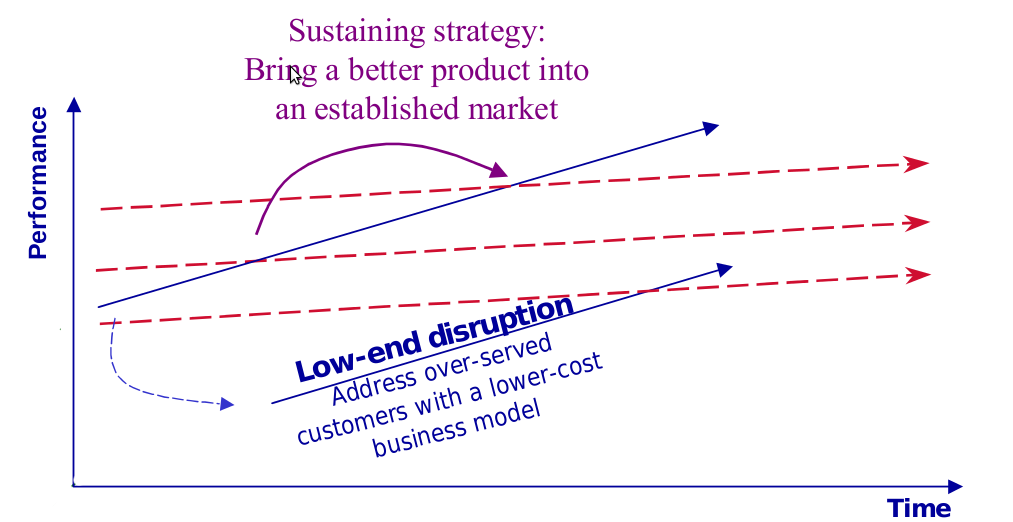
\includegraphics[width=0.9\textwidth]{images/simpleDisruptiveInnovationModel.png}
%\includegraphics{new_look_contents.png}
 \caption{The Disruptive Innovation Model (source: \cite{innovatorsSolution})}
\label{fig:disruptiveInnovationModel}
\end{figure}

The upper blue arrow represents the product performance growth over time. The sustaining innovations improve 
the product's "attributes most valued by the industry's mainstream customers" \cite{innovatorsSolution}, i.e. the drivers. 

However, according to the disruptive innovation theory, the pace at which companies improve their products by sustaining innovations is faster than 
the growth of customer sophistication - the ability to utilise or absorb improvements. 
This is illustrated by the stippled red lines in figure \ref{fig:disruptiveInnovationModel}. 
For example, a graphics card performance improvements 
beyond what is sufficient to play less demanding games does not effect low-end or casual gamers.

Over time, more and more customers become \emph{overserved}. The product becomes more complex and costly without valuable leverage for most customers. 
Despite this trend, the established company tend to continue doing what it has been optimized over the years to do: sustaining innovations.
The company has built internal and external structures that are optimized for competing in the high-end market, 
including its vision, processes, policies, assets, valued competencies/employees, corporate culture \cite{scientificArticlePredictingTheUnpredictable}, 
as well as its \emph{value networks} \cite{innovatorsDilemma}.
A value network is "the collection of upstream suppliers, downstream channels to market, 
  and ancillary providers that support a common business model within an industry." \cite{innovatorsDilemma}. 
That is, all its relationships and integrated processes with partners within the market.
This solidifies its position in the current market against any new entrant (e.i. startups), 
but at the same time makes it vulnerable for changes in the market, including changes in the priority of the dominant drivers.


This opens the door for \emph{disruptive innovations}, typically done by new entrants (i.e. startups) into the market with a new business model 
that can change the market significantly. \\

There are two types of disruptions, \emph{low-end} and \emph{new-market disruptions}, depending on the initial target customers.

In low-end disruptions, an entrant company starts by offering a product that is good \emph{enough} to the existing low-end market in regard
to the dominant driver, using a business model that enables profits at lower prices. 
Furthermore, the product might be better in regard to other characteristics as simplicity and convenience \cite{innovatorsSolution} 
making it a better choice for this market segment.
This is illustrated by the lower blue arrow in figure \ref{fig:disruptiveInnovationModel}.

The disruptor company is built around a new business model better suited for the low-end, which gives it the advantage.  
Instead of fighting back, the established company tend to abandon the unattractive low-end and focus on the more attractive high-end market, where it has
a competitive advantage. In the short term, this is more profitable, "feels good" and makes "perfect sense" \cite{innovatorsSolution}. 
Thus, the established companies ignore the eminent threat. 
However, as the disruptor begins its own cycle of sustaining innovations, it gradually improves the product in regard of the dominant driver 
and builds its value network to serve more needs in the high-end, 
thereby pushing the established companies upward in the market. 
This continues until the bulk of customers are 
attracted to the new entrant company, thereby disrupting the market. Because the bulk of the customers are usually concentrated in the 
middle of the sophistication scale, when the disruptor matures enough for the mainstream customers this results in a relatively 
quick and sudden market change. The old companies are either reduced to the high-end niche or disappear completely.


On the other hand, in a new-market disruption, the disruptor starts by offering 
typically a simpler, more convenient product to \emph{nonconsumers}.
Nonconsumers are persons that previously either could not afford, did not have the skills to use the products in the established 
market or did not find them convenient enough.
Thus, the new entrant company competes against "non-consumption", by offering a product to a whole new population that have had no alternative. 

For example, cell phones/mobiles opened the opportunity for casual gaming in situations where console or computer gaming wouldn't be practical 
(i.e. while waiting for a bus).

This type of disruption is the most frequent \cite{disruptionInEducation} and advisable for new entrants \cite{DisruptingClassExpandedEdition}. 
This is illustrated in figure \ref{fig:twoDisruptiveInnovationModels} by a new (green) plan.

\begin{figure}[here]
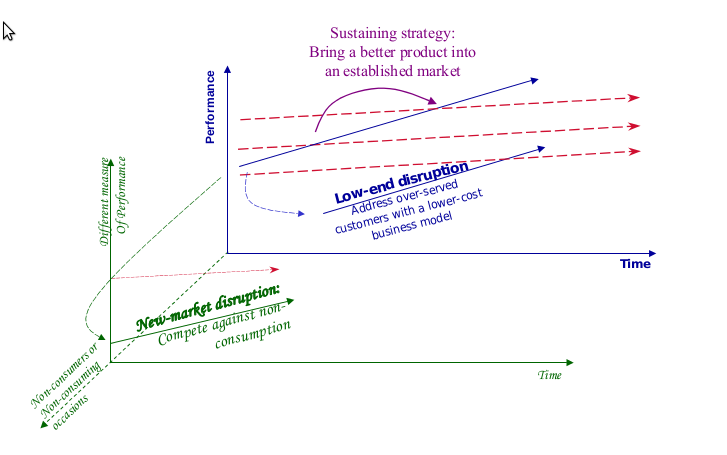
\includegraphics[width=0.9\textwidth]{images/twoDiruptiveInnovationModels.png}
%\includegraphics{new_look_contents.png}
 \caption{The Two Disruptive Innovation Models (source: \cite{innovatorsSolution})}
\label{fig:twoDisruptiveInnovationModels}
\end{figure}

Initially, the product is not sophisticated enough for the existing customers in the old market, 
and the performance is perceived differently in the new market (along other drivers). 
For example, graphics quality in mobile games was lower than console games but good enough for this niche, while offering convenience, simplicity and meaningful shorter
gaming sessions.

As in the case of low-end disruptions, the product improves gradually, and the niche market grows, attracting more interest, resources and competition.
This accelerates the sustaining innovation cycle within the new market, which is ignored by the established companies because it is 
perceived as another market, and it initially grows the overall industry instead.
However, the new market eventually pulls customers from the old market. This happens because the new players improved their 
product against the old drivers, a shift happened in the priorities of drivers or the old drivers became obsolete in the old market.\\


Employing disruptive strategies, both low-end, new-market or a combination thereof, many companies accross different industries 
have successfully overtaken markets \cite{innovatorsSolution}. For instance, when the Apple II computer was launched, it was too basic 
for the financial and engineering applications that used to be handled by minicomputers. Apple II was sold as "children's toy" thereby 
creating a whole new market that previously did not exist. 
As personal computers improved, they disrupted the minicomputer market \cite{disruptionInEducation}. 
\\

%With the continuous performance improvement of smartphones \cite{samsungCompetingAgainstPlaystation4}, the graphics and  gaming experience improved, with the mobility and social attributes 
Most successful disruptions have three enablers: 
a simplifying technology (makes it simpler and/or more convenient to do a job), a business model innovation (new definition of who the customers are, 
what is the value proposition, key processes and resources, and a profit formula \cite{reinvetingBusinessModel}), and a new disruptive 
value network \cite{pressArticleHbsReviveHealthCareInnovation}. 
A disruptor rarely disrupts the market alone, in that to efficiently replace 
the established market, a whole new network needs to arise \cite{DisruptingClassExpandedEdition}\cite{pressArticleHbsReviveHealthCareInnovation}. 
For example both the personal computers and smartphones need a whole ecosystem (software/apps, education/books, distributor channels etc) to thrive.
\\

Wether an innovation will disrupt a given market is difficult to predict \cite{innovatorsSolution}. 
However, even when established companies are aware of the threat and try to counter it, they often fail \cite{innovatorsSolution}. 
The reason is that companies cannot disrupt themselves \cite{innovatorsSolution} and diruptive initiatives get co-opted into sustaining innovations. 
The best strategy for established companies, according to Christensen, 
is to create a new business unit separate from the company, run under the same conditions as a startup \cite{innovatorsSolution}. 
% TODO check where "new biz unit instead of disrupting yourself"
Constantinos Markides goes as far as advising established companies to "not even attempt to create such innovations", but should leave the task 
to better suited startups, and instead aquire the successful ones and consolidate the new markets into big, mass markets \cite{scientificArticleDisruptiveInnovationBetterTheory}.

% Quote used:
%"established companies should not even attempt to create such in-novations but should leave the task of creating these
% kinds of markets to small, start-up firms that have the requisite skills and attitudes to succeed at this game.Established firms should, instead, concentrate on
%what they are good at—consolidating young markets into big, mass markets." \cite{scientificArticleDisruptiveInnovationBetterTheory}

In the next section, we look into the effectuation theory, that explains how expert entrepreneurs think and behave in the startup phase of their entrepreneurial quest,
and how it relates to the disruptive innovation theory.


\newpage

\subsection{The Effectual Entrepreneur}
In order to explain how entrepreneurs create new firms, Saras D. Sarasvathy proposed a new decision model \cite{effectuationProposal}, \emph{effectuation}, 
which she later established empirically by a series of experiments \cite{effectuationExperiment}.
27 expert\footnote{An expert entrepreneur in this study is a person who started one or more companies that have a value from 200 million to 6.5 billion USD}
entrepreneurs and 37 students (i.e. novice entrepreneurs) were given the task of creating a company from scratch.

Most students based their decisions on \emph{causal reasoning}. They proceed analytically with market research and competitor analysis 
to identify potential target customers from a predetermined market, and estimate expected returns. With a fixed goal (i.e. \emph{effect}) the students proceed then 
analytically to find the optimal sequence of events and the means necessary to \emph{cause} the effect. 
The implicit assumptions are that the market already "exist[s] independent of the firm", the future is predictable 
(plan to achieve a future effect and return, by a known series of events), and that any risk threatening the plan is bad and should be avoided.

Most experts, on the other hand, used an almost \emph{reversal} decision-model, called \emph{effectual}, illustrated in figure \ref{fig:effectualCycle}. \\

\begin{figure}[here]
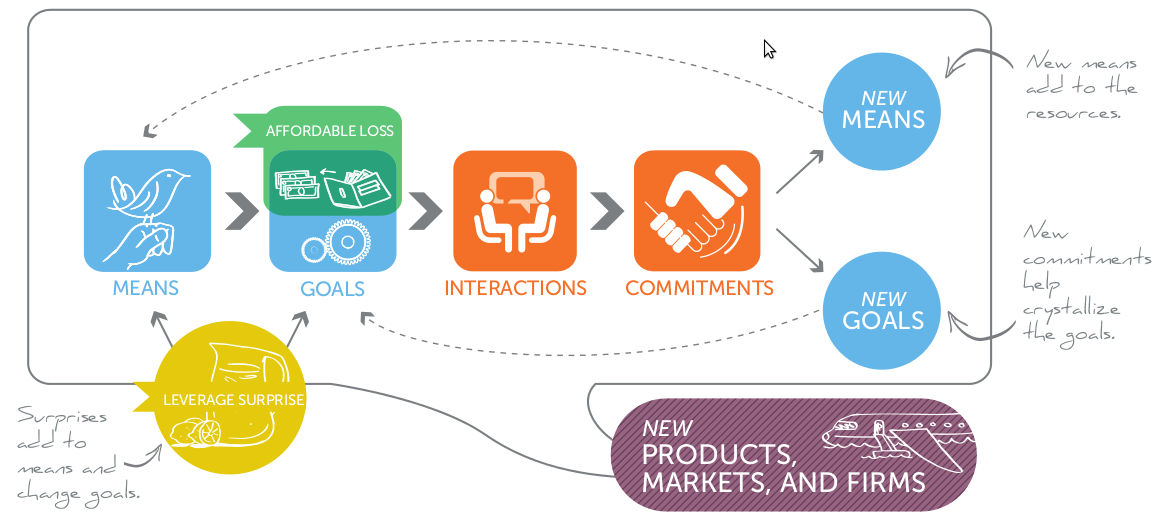
\includegraphics[width=1.1\textwidth]{images/effectuationCycle.png}
%\includegraphics{new_look_contents.png}
 \caption{The Effectual Cycle (source: \cite{effectualCycle})}
\label{fig:effectualCycle}
\end{figure}


With no rigidly fixed goal but only an aspiration, the experts ignore market research and competition. Instead, they start immediately with 
what they can do with the means they have and can afford to lose, thereby minimizing the risks. 
They do not predict if, but ensure there is demand for the product as quickly as possible. 
Starting from what and whom they know, they interact with people in their network and gradually aquire concrete customers and get commitments 
to the venture from partners. 
This fruitful interaction increases the means available, and possibly results in partners and customers influencing the flexible goals. 
This process is repeated iteratively, crystallizing the goals and increasing the network, until the experts end up by \emph{creating} a new market. 
There is no need in predicting the future, since the expert entrepreneurs shape it together with partners and customers.
If the unexpected happens, the experts take it as a hint of a possible opportunity and would try to adjust the path to take advantage of it instead of sticking to a rigid plan.
\\

There are five principles that govern the effectual decision-model:


\begin{enumerate}
 \item \emph{Bird in hand}: experts start with their means (who I am: traits, tastes and abilities; 
  what I know: education, training, expertise, and experience; and whom I know: social and professional networks) \cite{effectuationWhatMakesEntrepreneurial} 
  and imagine possibilities they can pursue. 
    That is, their choices reflect their personality, knowledge and network instead of rational analysis and prediction
 \item \emph{Affordable loss}: At each step, their efforts and choices are guided by what they can afford to lose, not by a projected future revenue
 \item \emph{Patchwork Quilt}: experts co-create a market with committed partners, spreading the risk, aquiring new means and crystallizing the goals
 \item \emph{Lemonade}: bad surprises give an opportunity to learn and give useful clues while creating the market
 \item \emph{Pilot-in-the-plane}: "the future is neither found nor predicted", but rather made and controlled 
\end{enumerate}


Although the goal is not fixed, "at any given moment, there is always a meaningful picture that keeps the team together, a compelling story that brings in more
  stakeholders ..." \cite{effectuationWhatMakesEntrepreneurial}.
  
Experts prefer effectuation, but recognize both causal and effectual reasoning as important, each in the appropriate context \cite{effectuationProposal}\cite{effectuationBook}.
In fact, both can be used simultaneously \cite{effectuationVideoEffectuationVsCausation}\cite{effectuationCausationEffectuationAndPragmatism}. 
For example, an entrepreneur can use a 
means-driven approach but still try to predict outcomes if the knowledge available permits to do so reasonably, 
or build partnerships while safeguarding intellectual property and being fully aware of competition when it makes sense \cite{effectuationCausationEffectuationAndPragmatism}.

In situations with high uncertainty, e.g. in a startup phase when commertializing an innovation, effectuation is particularly useful \cite{effectuationProposal}.
It helps reduce the costs of failure \cite{effectuation101}, in fact, "failing is an integral part of venturing well" \cite{effectuationBook} 
by early validation that keeps failures relatively small and an opportunity to learn \cite{effectuationNewVenturePerformance}\cite{effectuationBook}. 
Most importantly, effectuation helps to bring people (early customers, partners) on board \cite{effectuationVideoEffectuationVsCausation}, 
so much so that "system builder" has been proposed as a more descriptive name than
"entrepreneur", to reflect the importance of a systemic approach \cite{effectuationSystemicDesign}, i.e. bringing different parts and means together in a coherent network.

In a situation where knowledge permits a reasonable level of prediction, a more causal approach would be appropriate \cite{effectuationNewVenturePerformance}. 
For example, as a market begins to emerge and a product or business model begins to work \cite{effectuationNewVenturePerformance}. 
In fact, a causal approach is necessary for scaling (expanding) the business after the business model has been validated \cite{effectuationVideoEffectuationVsCausation}.


\subsubsection{Link to disruptive innovation}
Despite that research linking disruptive innovation and effectuation is minimal \cite{managingDisruptiveInnovation}, there seems to be an obvious overlap.
As seen in the previous chapter, Christensen advises to start disrupting a market by creating a new market, and 
disruptions rarely occur without a creation of a whole new value network that can disrupt the old. 
Effectuation is especially helpful in creating new markets and building partnerships.  

There is high uncertainty when creating a new market, that makes it unknowable what product design/features for what customer/partners 
would work \cite{effectuationDisruptiveInnovationBusinessDevelopmentMarketing}. Examples of \emph{exaptation}, the successful use of innovations 
in markets they were not intended for when first developed, are numerous  \cite{managingDisruptiveInnovation}.\\
Exploratory (or experimental) approaches have been proposed to test different permutations of product features early on to different customers until a match is found
with a viable business model \cite{managingDisruptiveInnovation}\cite{effectuationDisruptiveInnovationBusinessDevelopmentMarketing}. 
Despite the uncertainty, \emph{Business Development}, an effectual exploratory approach proposed specifically for disruptive innovations, combines 
some causal aspects as market analysis to identify potential partners and customer segments to explore. In particular, it encourages the engagement and 
exploration of potential partners, e.g. distribution channels, in the early phase in a systematic way \cite{effectuationDisruptiveInnovationBusinessDevelopmentMarketing}.

In addition to iteratively assessing different features permutations with customers in real life settings, opening a direct channel to tap into user ideas, 
for example an online platform, can be a fruitful initiative to generate disruptive innovations \cite{managingDisruptiveInnovation}.



\subsection{The Consistent Startup}
With the aim of understanding what makes startups succeed or fail, the team behind the Genome project processed
data from more than 3200 "internet startups" to identify commonalities between successful startups.

Startups are described as 
\begin{quote}
\emph{"temporary organizations designed to scale into large companies.
Early stage startups are designed to search for product/market fit under
conditions of extreme uncertainty. Late stage startups are designed to search for
a repeatable and scalable business model and then scale into large companies
designed to execute under conditions of high certainty."} \cite{genomePrematureScalingReport}
\end{quote}	
That is, a startup's primary mission is to learn and discover a product that fits the needs of a (new) market, 
that can be met profitably in a repeatable and scalable way.

A startup has five dimensions that need to grow simultaneously.
"a developmental organism that evolves along 5 interdependent dimensions: Customer, Product, Team, Business Model and Financials." \cite{genomePrematureScalingReport}
(more...)

The most fundamental insight gained, is that successful high growth startups manage to grow all dimensions in a consistent way.
(more...)

A high growth startup goes typically through a lifecycle \cite{genomePrematureScalingReport} described below

\subsubsection{Startup Lifecycle}
A high growth startup goes through 4 stages until it reaches "scale", as shown in table \ref{fig:startupLifecycle}:

\begin{center}
\begin{table}
  \begin{tabular}{ | l | p{5cm} | p{6cm} | p{1.8cm} | }
    \hline
    Stage 	& Purpose 						& Events	& Time \\ \hline
    Discovery 	& Validating the problem and whether anybody would hypothetically be interested in
		  the solution.
		& Founding team formed, customer interviews,
		  value proposition is found, minimally viable products are created, team joins an
		  accelerator or incubator, Friends and Family financing round, first mentors and
		  advisors come on board.		& 5-7 months \\ \hline
    Validation 	& Early validation that people are interested in
		  the product through the exchange of money or attention.
		& refinement of core features, initial user growth, metrics and analytics
		  implementation, seed funding, first key hires, pivots (if necessary), first paying
		  customers, product market fit.	& 3-5 months \\ \hline
    Efficiency 	& Refining business model and improving the efficiency of 
		  customer acquisition process. Startups should be able to efficiently acquire
		  customers in order to avoid scaling with a leaky bucket.
		& value proposition refined, user experienced overhauled, conversion
		  funnel optimized, viral growth achieved, repeatable sales process and/or
		  scalable customer acquisition channels found.	& 5-6 months \\ \hline		  
    Scale
		& Startups step on the gas pedal and try to drive growth very aggressively.
		& Large A Round, massive customer acquisition, back-end scalability
		  improvements, first executive hires, process implementation, establishment of
		  departments.		& 7-9 months \\ \hline


    \end{tabular}
    \caption{Startup lifecycle (Source: adapted from \cite{genomeOriginalReport}) \label{fig:startupLifecycle}}
  \end{table}
\end{center}

In the first stage, the startup discovers the . Then validating that it users consistently use/buy the product, makes sense.







\begin{enumerate}
 \item Forget products/market segments, it is all about jobs-to-be-done: the roots why people "hire" a product \cite{reinvetingBusinessModel}
       Note: Effectuation: people do not use time on market research - they create the market!
 \item "People don’t want a quarter-inch drill—they want a quarter-inch hole."
 \item Established or big companies are adviced to create a separate startup like unit.
\end{enumerate}

 
 
A startup anology that works well, is organ development in early stages. 
Need to grow harmoneously between all dimensions of startup, until it reaches a final shape;
And find itself/identity to form and adapt to how to serve a specific need/market-to-be.
Then it can grow on this foundation.

According to Genome types, Padness is "The Social Transformer / Type 1N" (social reading/studying)

 - Clayton: understanding jobs to be done is the starting point, build everything upon it \cite{reinvetingBusinessModel}

So, as Disruptive Innovation sais about jobtobedone and forge the whole based upon, organ has to form itself. Ok

Findings:
"Startups need 2-3 times longer to validate their market than most founders
expect. This underestimation creates the pressure to scale prematurely"

"Startups are temporary organizations designed to scale into large companies.
Early stage startups are designed to search for product/market fit under
conditions of extreme uncertainty. Late stage startups are designed to search for
a repeatable and scalable business model and then scale into large companies
designed to execute under conditions of high certainty."

The Organic Startup
 How should IT-startups do it? Jobs-to-be-done is discovered and startup builds around it and a business model, and grow organically
 to be a grown up company.
 A balance excercice between all aspects of the startup
 
 
 ---
 "I believe the missing piece from the DNA in the founding teams of 
  Transformational Companies is now the Domain Expert, 
  who has deep insight into the industry they are trying to disrupt. "
 \url{http://blog.startupcompass.co/reversing-the-decline-in-transformational-ide}\\

 Genome, orig. report
 "Technical teams did very well with Type 1 (The Automizer) startups and didnot do very well with Type 1N (The Social Transformer) startups"
% http://www.scribd.com/fullscreen/56508265?access_key=key-2lfkcv2ysdvb43cwmfx7
 
\subsection{Pretotyping}
Matches great, and the Agile movement/Lean startup
Early stage: pretotyping find the job(s) to be done
\\
Interpretation: shorten the speculative phase and back it up with user data
\begin{enumerate}
\item iteration, 
\item AB test, Google made millions of \$ on changing link blue color shades to figure best.
\item data collection, 
\item metrics, 
\item one or more projects
\item Continuous deployment
\item First disable caching, to get most hits, then enable if necessary
\end{enumerate}

Small AB tests, too much to require users to install and reinstall different
Early stage development: Minimum Viable Product pretotyping
 - What pretotyping is
  --- beware vanila metrics, i.e. user growth if no revenue stream.
 - beta, alpha
 - AB/split test
 - Requires Quick development/deployment
 



\subsubsection{Challenges of pretotyping on thick clients}

---
http://hbswk.hbs.edu/item/6659.html
Tom Eisenmann, a professor in the Entrepreneurial Management Unit at Harvard Business School.

"Lean startups don't try to scale up the business until they have product market fit [PMF], a magical event—more 
 easily recognized in retrospect than in the moment—when they finally have a solution that matches the problem"
----

To be Quick is fine, but needs flexibility to change. However, backward compatibility imposed, delays might incur etc.
Needs to reverse quick bad decisions. Keep control over architecture (well behaved clients).
 * Challenges of thick client pretotyping
 - Client distribution out of control: external distributor. Sometimes restrictions/rejection, delays in distributing update etc.
 - unflexible for pretotyping practice (cons)
    - For example if one makes a quick pretotype with heavy polling, then it shows to be too much, not possible to easily retire the client.
   not easy AB test: no full control over installs. 
 - In beginning, important to convey a good image and make to be a "sticky" app in the users mind. Before that, don't annoy/expect user
   with too many re-installs
 - Forced external API Design (cons but make it advantage - prepare platform API, and possible easier partnership)
    API deprecation, reverse wrong design: keep control over system
 - Architecture: 
    Cost and difficulty when time passes, for website, even more when no control over a component in the architecture:
      change in Design --costs(++)--> Impl.
      scala+perf. most difficult to adjust. Anecdote: Amazon split server for Christmas season. Might have had significant concequences.
    performance, scalability and reliability (advantage thick client computation available)


Communication with users
AB test

\subsubsection{public API trend, and platform a good way to go}
A public API is a way to build an eco system around a product/service, it is a trend and should be envisaged.
However, API's as stars in the universe, inchangeable and will be wrong first time.
Prepare for evolution, deprecation.
So, my own note: use it internally before public, eat you own food.

\subsection{Architecture}
Although probability low, and many focus on scalability too early, bad if chance goes away and we are here for high growth systems anyway.
So, make lightweight decisions that keep my system open for scalable solutions in the future with relatively small price.

Keep all possibilities open, open evolvable architecture for different loads.
\begin{enumerate}
\item Design costs less, after costs more...
\item Scalability and performance are most difficult to add as an afterthought
\item An architecture that both satisfies the needs of the pretotype in early stage, but can evolve
    into a scalable solution
\item QRCS read-write separation
\end{enumerate}

Client loadbalancing.
Cloud more expensive than own. Cloud not good at scalability; cannot optimize (commodity), [not near CPU, LMAX architecture,...].
Plus, cost saving in beginning important. Investment postponed, but success needs most of hardware investment, so best:
Client load balancing, hybrid cloud-hosting.

\section{Approach}
A (3osarat) resume is to:
- start from what one have: I am arab, student, know educators and publishing houses in arab world, have access to copyright free books
- niche good, focus.
- build basic seed add what opens different types of partnerships: investors (collect data, but disable if too much), authors (feedback), 
self-authors (+corrections), schools (teacher<->students<->students), publishers (correction, usage stats), software houses cooperation.

--- in the light of education disruption

- make lightweight architecture (remote control, API Design, scalability if it comes)
-- separate client from server, enable each to evolve 
-- separate backend by two dimensions: 1) services, 2) read-write
- launch then look for partnerships with concrete product and user numbers (more credibility with product in hand)
- Hold eye on growth: if scale, move to arch, otherwise optimize user experience, user retention, feedback loops etc. until it takes off.
- continuous integration/deployment, test. However, might be too complicated if simple backend, introduce when necessary.


\section{Case}
\subsection{Use cases}
\begin{enumerate}
\item Easy corrections
\item Class mate and group reading
\item Asking clarifications from author
\item Author understanding of book unclear passages, reading patterns etc. to improve book
\item Author More data about how book is read, time spent etc.
\end{enumerate}
 
 IDEAs: 
 - ebooks that change depending on type of user learning preferences (?)
 - MEAP/Manning: books dev-loop and sold. What about more dynamic, realtime feedback loop?
 
 
 Disruption in Education, paper:
-----------------------------------

" The CDs often were left in their jackets and the
Web sites were rarely visited. Had the publishers observed stu-
dents, they would have found that what students really do is
wait until the last minute to read their textbooks. What they
really need is a way to help them learn quickly right before an
exam and the ability to 
*************************
share class notes online.
*************************"


---
http://www.educause.edu/ero/article/role-disruptive-technology-future-higher-educational

"Terry Anderson12 pointed to the importance of placing the student at the center of the learning experience, as have others.
 That means a greater focus on student-generated content, students’ use of collaboration and sharing tools such as Web 2.0 applications, and modular tutoring."

"... automated instruction, self-publishing, and peer-to-peer networking."

\subsection{Applying disruption approach}
A successful disruption of print books can reach far beyond the publishing industry.

Textbooks are a cornerstone in the education system, and its creation and distribution is the first activity in 
the chain of activities that together constitute the public education's 
\emph{value network} \cite{DisruptingClassExpandedEdition}. A \emph{value network} comprises all activities by different partners, 
suppliers and channels that together serve particular customers.

The US education system is becoming too expensive \cite{theInnovativeUniversity}. 
With continuously increasing tuition fees \cite{risingTuitionFees}\cite{theInnovativeUniversity} and student debt 
reaching a staggering 1 trillion USD in the US \cite{oneTrillionUsStudentDebt}, the education market is in need of 
more affordable alternatives. Combined with a fundamental mismatch between the unique individual student learning 
preferences and the increased standardization of education \cite{DisruptingClassExpandedEdition}\cite{educationInnovationNecessaryForEconomicGrowth}, 
the education industry is itself ready for disruption \cite{DisruptingClassExpandedEdition}\cite{theInnovativeUniversity}.

Indeed, the disruption might already have started. In recent years, online course enrollment in the US has increased 
"substantially faster than overall higher education enrollments" \cite{babsonOnlineEduGrowth2011}. Specifically, online 
enrollments growth rate has been more than ten times the growth rate of overall higher education enrollments in the fall 2010. 
31 percent of all higher education 
students take at least  one course online, and 67 percent of academic leaders rated the learning outcomes 
"as the same or superior to those in face-to-face" \cite{babsonOnlineEduGrowth2011}. 
Clayton M. Christensen, a leading expert in disruptive innovation theory, predicts that by 2019,
fifty percent of all high school courses will be delivered online \cite{DisruptingClassExpandedEdition}.

However, a disruptive online education, or more generally computer-based learning, is not a mere replication of the monolithic 
"bricks and mortar" education online \cite{DisruptingClassExpandedEdition}. Despite heavy investment in computer systems, previous attempts have 
largely failed to deliver significant improvements, because the technology has been co-opted to the existing teaching model, serving 
existing students \cite{DisruptingClassExpandedEdition}. 
Instead, to be successful, a new student-centric teaching model ducational system 
about using a new tool to deliver the same monolithic experience, 
but rather
There are interesting innovations in online education, including Coursera's Massive Open Online Courses (MOOC), some of which 
and khan translated to more than 50+ languages. It is appealing to an international audience (not just the US).
Education is competitiveness, 
With a global education spending of 4 trillions USD per year predicted to double by 2020 to 8 trillions USD...
In this innovation thesis, I am initially asked by a startup to build an eReader application for Android. With this fast paced ebook and educational market,
ambitions quickly got higher - eReaders are more than books. Not only digitize the reader. Interconnected, powerful devices.
However, startups fail, and even established companies.

So, need learn big picture, deduce requirements for process and architecture.

Many educational startups emerged in recent years \cite{boomEducation1}\cite{boomEducation2}, as well as big players like Apple, Intel, 
Google and Microsoft battling for the education market. The estimated global spending on education is about 4 trillion USD, projected to grow to
8 trillions USD by 2020.

Massive Open Online Courses (MOOC), courses with large scale student participation from few thousands to hundreds of thousands of participant 
in a given course.


Nation competitiveness. But not standardized, customized, user sharing etc.



Findings applied to education 
(Note: IT disrupting education, not only iPads. But iPads/eReaders disrupting books -> disrupting textbooks used in education?)
\begin{enumerate}
 \item Traditional way of education is too inflexible, standardized, students run in batches, subjects and departments are silos
 \item People learn differently, different paces, different interests and capabilities 
 \item Learning best by creating and engagement two-ways or peer-to-peer, not one-way-hearing \cite{disruptiveOrLiberatingEducation}
 \item Creativity comes at cross-roads of different disciplines 
 \item " ...schools.. online learning programs failed simply because they tried “to provide traditional courses in a nontraditional manner.”"
 \item " Attempting to market an inferior product to their most demanding customers was, predictably, a recipe for failure"
 \item "...problem was that they were still competing against consumption."
 \item is ready for disruption
\end{enumerate}


-----------
Rita Kop, “Web 2.0 Technologies: Disruptive or Liberating for Adult Education?” Adult Education Research Conference 2008, St. Louis, Missouri, June 5–7, 2008.
  
Students need to create content, get it validated by peer (Tayeb: voting?) and expert feedback.
Free to construct, but get validated instead of one-way-hearing. Maybe not fully understand until validating ones own thoughts?
Get knowledge from different sources, no time/space limits. Chaos, creativity.

"... people take ownership of the learning process, rather than institutions controlling their education"

"... they preferred the online
mode of study, which is flexible and available at the time and place to suit them and fitting in
with their lifestyles better than face to face teaching, [but] they required a lot more nurturing than
anticipated. "
-----------

conclusion:?
Courses with lots of books, deep\\
Non-consumers(non-students): Books, "randomly chosen", by topic, on your own.\\
Offer: Package mini courses with the books in one package, peer-to-peer.!
\\
But how do expert do it?


\subsubsection{Applying effectuation (remove?)}
Apply
\begin{enumerate}
 \item Pilot in the plane: "the future is neither found nor predicted", but rather controlled 
 \item Bird in hand: apply:(arabic books, understand language and culture, network; P.inc servers) - and find and do what is doable.
 \item Affordable loss: my time for thesis, P.inc: limited funds for Amazon, Google play etc. 
 \item Partnership: (now move to k12 with iqra school instead of university-wish-to-be)
 \item Leverage surprises: Use uncertainty to own benefit, investors doubted: further develop concept etc.
\end{enumerate}

\subsection{Why/strategy}

 Arabic Niche, Low cmompetition, hope for higher interaction
 iOS success, demand for android

\subsection{Possible paths and what should be done in each case}
If high growth, move to scalable
If low growth, work on customer aquisition and retention
Enhance existing functionality
Add functionality 

\subsection{What happened}
Pretotype with HTML5 (titanium), made book scanner. However too slow.
Some big companies that used it, moved away from it.


In beginning, a thought of developing API, let existing iOS app be enhanced with interaction to get feedback quickly, start immediate iteration
However, problems with external devs, genome sais it!
Dropped and moved to android

Web (minimum), failed, parked
Android: basic has to be in place, pretotype only on new extra features. Challenge


Need fast desicion, product owner present or autonomy.
Authority to decide

\subsubsection{Implementation}
\subsubsection{Arabic}
Arabic letters different forms. Needs reshape. Had an open source starting point, but had bugs for some letters, and no "tashkeel".
Bug long lines, sometimes letters inversed.
Need to estimate line length and cut.

Search: trade off, between size, speed and batteri. Chose speed and batteri - space can be purchased.
word reshaped before indexed - remove tashkeel.


\subsubsection{Log analysis}

\begin{enumerate}
\item Although arguably less user friendly, number of user contents available per page is not available. Interested users would click on it, so
we register interest even if most books have no annotations in the beginnning. Not enough resources to enter/sponsor/encourage initial user 
content.
\item various books different interests, too scattered user annotations. To get momentum, needs focus user groups, for example cooperate on 
particular course and get students to interact with each other and teacher through app to add content. Otherwise, users are disappointed.
\item Remarked same users click on different pages from same book, guess frustrating, especially when most have no content, 
so made change added different categories: page, chapter and book.
\item Quite few users attempted repeatedly to login but failed, even after successful registration with arabic names. A bug hindered UTF8 
usernames from client side. Was too cumbersome to fix with time limit. Others tried with email. Quick fix was to send message, 
meanwhile made stricter client validation: no arabic, no email.
\item Quite few failed registration because of weak password. The numbers were quite significant, and turned out they used numbers only password.
Restriction was removed.
\item In general, we need a much easier user account creation and login process, possibly with auto picking user (Google) email if available
and generating a password so user only needs to approve.
\end{enumerate}

\subsection{Requirement and architecture}
Prepare for scalability, even not implementing:
\begin{enumerate}
\item Avoid bottleneck on id generator
\item Shard-able ID creation, one per book well defined algorithm
\item Scalability and performance are most difficult to add as an afterthought
\item An architecture that both satisfies the needs of the pretotype in early stage, but can evolve
    into a scalable solution
\end{enumerate}


\section{Conclusion}


\begin{thebibliography}{9}


%@article{christensen2003disruption,
%  title={Disruption in education},
%%  author={Christensen, C.M. and Aaron, S. and Clark, W.},
%  journal={Educause Review},
%%  volume={38},
%  pages={44--55},
%  year={2003},
%  publisher={EDUCAUSE}
%}

%)

\bibitem{pressArticleStartupsFailure75percent}
  \emph{Study: Most venture-backed technology startups fail }\\
  \url{http://money.msn.com/investment-advice/latest-4.aspx?post=0b0cb8cb-199d-4112-bef8-71a9d1c1a07d}\\
  (Accessed 22 December 2012)\\
  
  
  
\bibitem{pressArticleStartupsFailureUpTo95percent}
  \emph{Why Companies Fail--and How Their Founders Can Bounce Back}\\
  % 2011
  \url{http://hbswk.hbs.edu/item/6591.html}\\
  (Accessed 22 December 2012)\\
  

\bibitem{disruptiveOrLiberatingEducation}
  Rita Kop, \\
  “Web 2.0 Technologies: Disruptive or Liberating for Adult Education?” \\
  Adult Education Research Conference 2008, \\
  St. Louis, Missouri, June 5–7, 2008.

\bibitem{innovatorsSolution}
   Clayton M. Christensen, Michael E. Raynor,\\
   \emph{The Innovator's Solution: Creating and Sustaining Successful Growth},\\
   September 2003 \\
   Harvard Business School Press\\
 
\bibitem{disruptionInEducation}
   Clayton M. Christensen, Sally Aaron, William Clark\\
   \emph{Disruption In Education}\\
    2001\\
   \url{http://www.educause.edu/Resources/DisruptioninEducation/158712}\\

    
\bibitem{DisruptingClassExpandedEdition}
   Clayton M. Christensen, Curtis Johnson, Michael B. Horn\\
   \emph{Disrupting Class, How disruptive innovation will change the way the world learns, Expanded Edition}\\
    May 14, 2008\\
    Mc Graw Hill\\

\bibitem{articleDisruptingTextbooksInHigherEducation}
  Disrupting Tree-Textbooks in Higher Education\\
  Daniel Falabella, Salvael Estrada\\
  \url{http://byuia.com/innovation-and-the-academy/}\\
   (Accessed 22 December 2012)

\bibitem{scientificArticlePredictingTheUnpredictable}
  \emph{PREDICTING THE “UNPREDICTABLE”\\
  ANTICIPATING DISRUPTIVE INNOVATION}
  Jay Paap and Ralph Katz\\
  Research-Technology Management, 2004\\ 

\bibitem{scientificArticleDisruptiveInnovationBetterTheory}
  \emph{Disruptive Innovation: In Need of Better Theory}\\
  Constantinos Markides\\
  The Journal Of Product Innovation Management, 2006\\


\bibitem{onePointThreeMillionAndroidDeviceActivationPerDay}
  Eric Schmidt: “There Are Now 1.3 Million Android Device Activations Per Day”
  %\url{	
   http://techcrunch.com/2012/09/05/eric-schmidt-there-are-now-1-3-million-android-device-activations-per-day/
   %}\\
   (Accessed 15 December 2012)

\bibitem{risingTuitionFees}
 \emph{Tuition Rising: Why College Costs So Much} \\ 
 R. G. Ehrenberg\\
 Harvard University Press, 2002.
 
\bibitem{reinvetingBusinessModel} 
  \emph{Reinventing Your Business Model} \\
  Clayton M. Christensen, Mark W. Johnson, Henning Kagermann\\
  Harvard Business Review, 2009\\
 
\bibitem{theInnovativeUniversity}
 The Innovative University \\
 Changing the DNA of Higher Education From the Inside Out \\
 Clayton M. Christmas, Henry J. Eyring
 Jossey-Bass, 2010
 
 \bibitem{oneTrillionUsStudentDebt}
  %\url{	
 http://www.bbc.co.uk/news/business-20663550
   %}\\
 (Accessed 17 December 2012)

\bibitem{pressArticleHbsReviveHealthCareInnovation}
  \emph{How to Revive Health-Care Innovation}\\
  \url{http://hbswk.hbs.edu/item/6095.html}\\
  (Accessed 23 December, 2012)\\
 

\bibitem{pressArticleIpadDisruptingPcAndGaming}
IPad, tablets clearly disrupting PC market, survey finds\\
\url{http://bgr.com/2011/04/12/ipad-tablets-clearly-disrupting-pc-market-survey-finds/}\\
  (Accessed 23 December, 2012)\\
 
\bibitem{babsonOnlineEduGrowth2011}
  \emph{Going the Distance: Online Education in the United States 2011}\\
  I. Elaine Allen and Jeff Seaman\\
  BABSON Survey Research Group\\

\bibitem{boomEducation1}  
  \emph{Boom time for higher education startups}\\ 
  July 26, 2012,\\
  \url{http://www.oregonbusiness.com/linda/7830-online-higher-education-startups-boom}\\
  (Accessed 21 December, 2012)\\

\bibitem{boomEducation2}  
  \emph{Anticipating a Blended Classroom Boom Led by Education Startups}\\ 
  August 31, 2012,\\
  \url{  http://techcrunch.com/2012/08/31/blended-classroom-boom-education-startups/}\\
  (Accessed 21 December, 2012)\\

\bibitem{courseraTedTalk}
What we're learning from online education \\
Daphne Koller\\
\url{http://www.ted.com/talks/daphne_koller_what_we_re_learning_from_online_education.html}\\
  (Accessed 21 December 2012)

 \bibitem{microsoftInvestInNook}
   \emph{Microsoft Hooks Onto Nook}\\
   \url{http://online.wsj.com/article/SB10001424052702303916904577375502392129654.html}\\
   (Accessed 21 December 2012)
   
 \bibitem{subtextGoogleInvested}
 \emph{Subtext Raises \$3 Million From Google Ventures \& More To Make eBook Reading Social}\\
 \url{http://techcrunch.com/2011/10/25/subtext-raises-3-million-from-google-ventures-more-to-make-ebook-reading-social/}\\
   (Accessed 21 December 2012)
 
 \bibitem{rethinkBooks}
  \emph{Rethink Books Gives Us A Glimpse At Social Books (Video Demo)}\\
  \url{http://techcrunch.com/2010/11/11/rethink-books-social/}\\
  (Accessed 21 December 2012)
  
 \bibitem{startupEbookInkling} 
   \emph{Inkling raises \$17 million – Swings for the Fences}\\
   \url{http://www.edukwest.com/inkling-raises-17-million-swings-for-the-fences/}\\
 (Accessed 21 December 2012)
 
 \bibitem{startupEbookChegg}
   \emph{Chegg eTextbook Reader launches today – Works on any Device}\\
   \url{http://www.edukwest.com/chegg-etextbook-reader-launches-today-works-on-any-device/}\\
 (Accessed 21 December 2012)
 
 \bibitem{startupEbookKno}
   \emph{Intel Capital Leads \$30 Million Funding of Education Startup Kno}\\
   \url{http://www.bloomberg.com/news/2011-04-08/intel-is-said-to-lead-30-million-funding-of-education-tablet-startup-kno.html}\\
  (Accessed 21 December 2012)
   
 \bibitem{nytimesAmazonEbookSurpassedPrint}
  \emph{E-Books Outsell Print Books at Amazon}\\ 
  May 19, 2011,\\
  \url{http://www.nytimes.com/2011/05/20/technology/20amazon.html}\\
  (Accessed 19 March, 2012)\\

\bibitem{adultEbookSecondLargestBookFormat}
   \emph{Trade Sales Rose 13\% in January-June Period, AAP Says } \\
  \url{http://www.publishersweekly.com/pw/by-topic/industry-news/financial-reporting/article/54372-trade-sales-rose-13-in-january-june-period-aap-says.html}\\
  (Accessed 17 December, 2012)\\
  
  
 % "official effectuation"
    
\bibitem{effectuationProposal}
  \emph{Causation and Effectuation: Towards a Theoretical Shift From Economic Inevitability to Entrepreneurial Contingency}\\
  Saras D. Sarasvathy\\
  Academy of Management Review, 2001\\

\bibitem{effectuationBook}
  \emph{Effectuation: Elements of Entrepreneurial Expertise}\\
   New Horizons in Entrepreneurship Series\\
   Elgar, Edward Publishing, Inc. (May 1, 2009)\\

\bibitem{effectuationWhatMakesEntrepreneurial}
  \emph{What Makes Entrepreneurs Entrepreneurial?} 
  Saras D. Sarasvathy\\
  \url{http://www.effectuation.org/sites/default/files/What\%20makes\%20entrs\%20entl\%20note.pdf}\\
  (Accessed 27 December 2012)\\
  
\bibitem{effectuationNewVenturePerformance}
  \emph{New Venture Performance}\\
  Saras D. Sarasvathy\\
  \url{http://www.effectuation.org/sites/default/files/documents/2-ways-new-venture-performance.pdf}\\
  (Accessed 22 December 2012)\\
  
\bibitem{effectuation101}
  \emph{Effectuation 101}
  \url{http://www.effectuation.org/learn/effectuation-101}\\
  (Accessed 28 December 2012)\\

\bibitem{effectualCycle}
  \emph{The Five Principles and the Effectual Cycle}\\
  Saras D. Sarasvathy\\
  \url{http://www.effectuation.org/sites/default/files/documents/effectuation-3-pager.pdf}\\
  (Accessed 27 December 2012)\\
  
\bibitem{effectuationVideoEffectuationVsCausation}
  \emph{Sarasvathy - effectuation vs. causation}\\
  Saras D. Sarasvathy\\
  \url{http://www.youtube.com/watch?v=hCMpd7z4AbA}\\
  (Accessed 27 December 2012)\\
 
 % critiques
 
\bibitem{effectuationSystemicDesign}  
  \emph{TEDxOxbridge - Marc Ventresca - Don't Be an Entrepreneur, Build Systems}\\
  \url{http://www.youtube.com/watch?feature=player_embedded&v=l9T3diyqRPg#!}\\
  (Accessed 28 December 2012)\\
 
\bibitem{effectuationDisruptiveInnovationBusinessDevelopmentMarketing}  
  \emph{Business development in the early stages of commercializing
      disruptive innovation: considering the implications of Moore’s life
      cycle model and Christensen’s model of disruptive innovation}\\
  Joseph Giglierano, Robert Vitale, J.J. McClatchy\\
  Innovative Marketing, Volume 7, Issue 2, 2011\\
  

\bibitem{effectuationCausationEffectuationAndPragmatism}
  \emph{New Technology-Based Firms in the New Millenium\\
	Chapter 13:  The Nature of the Entrepreneurial Process: Causation, Effectuation, and Pragmatism}\\
    Jeroen Kraaijenbrink\\
    Emerald Group Publishing, 2012\\
  \url{http://www.emeraldinsight.com/books.htm?issn=1876-0228&volume=9&PHPSESSID=5quega043s5ab8tjno37jo9220}\\
  (Accessed 28 December 2012)\\

  
\bibitem{disruptiveInnovationToBusinessModelInnovation}
  \emph{From Disruptive Technology to Disruptive Business Model Innovation: In Need for an Integrated Conceptual Framework}\\
  Solomon R. Habtay, Magnus Holmén\\
  \url{http://www.aomevents.com/media/files/ISS\%202012/ISS\%20Parallel\%20Sessions\%20/Habtay.pdf}\\
  
\bibitem{managingDisruptiveInnovation}
  \emph{MANAGING DISRUPTIVE INNOVATION: ENTREPRENEURIAL STRATEGIES AND TOURNAMENTS FOR CORPORATE LONGEVITY}\\
  Yanto Chandra, Shu-Jung Sunny Yang\\
   Journal of General Management, November 2011\\
  \url{http://papers.ssrn.com/sol3/papers.cfm?abstract_id=1965000}\\
  (Accessed 27 December 2012)\\

  
 % Genome
 
 
\bibitem{genomeOriginalReport}
  \emph{Startup Genome Report\\
	A new framework for understanding why startups succeed}\\
    Max Marmer, Bjoern Lasse Herrmann, Ertan Dogrultan, Ron Berman\\
    Startup Genome\\
  \url{http://blog.startupcompass.co/pages/startup-genome-report-1}\\
  (Accessed 28 December 2012)\\

\bibitem{genomePrematureScalingReport}
  \emph{Startup Genome Report Extra: Premature Scaling\\
	A deep dive into why most high growth startups fail}\\
    Max Marmer, Bjoern Lasse Herrmann, Ertan Dogrultan, Ron Berman\\
    Startup Genome\\
  \url{http://blog.startupcompass.co/pages/startup-genome-report-extra-on-premature-scal}\\
  (Accessed 28 December 2012)\\

  
\bibitem{genomeStartupDefinitionNotDone}
  \emph{How do you define a “startup”?}\\
    Max Marmer, Bjoern Lasse Herrmann, Ertan Dogrultan, Ron Berman\\
    Startup Genome\\
  \url{http://blog.startupgenome.com/how-do-you-define-a-startup/}\\

  % old order of refs
  
  \bibitem{1}
   \emph{eBook Market Exploding, Confirms New IDPF Survey}\\
   \url{http://www.huffingtonpost.com/mark-coker/ebook-market-exploding-co_b_507107.html}\\
  (Accessed 19 March, 2012)\\

\bibitem{2}
   \emph{Why E-Books are Hot and Getting Hotter}\\
  \url{http://www.huffingtonpost.com/mark-coker/why-e-books-are-hot-and-g_b_320986.html}\\
 (Accessed 19 March, 2012)\\

\bibitem{3}
   According to the following iTunes stats, 20 percent + of active applications are either books or education related \\
   \emph{App Store Metrics}\\
   (Page last updated: 2012-02-13 06:00:09 -0800 PST): \\
   \url{http://148apps.biz/app-store-metrics/?mpage=catcount} \\
  (Accessed 19 March, 2012)\\
 
\bibitem{4}
   \emph{The Rise and Rise of e-Textbooks [Infographic]}\\
   \url{http://www.getelastic.com/the-rise-and-rise-of-e-textbooks-infographic/}\\
  (Accessed 19 March, 2012)\\

\bibitem{amazonEbookSurpassedPrint}
  \emph{That Was Fast: Amazon's Kindle Ebook Sales Surpass Print (It Only Took Four Years)}\\
  \url{http://techcrunch.com/2011/05/19/that-was-fast-amazons-kindle-ebook-sales-surpass-print-it-only-took-four-years/}\\
  (Accessed 20 March, 2012)\\




\bibitem{barnesEbookPassPrint}
  \emph{Barnes \& Noble: eBooks will pass print -- fast}\\
  \url{http://tech.fortune.cnn.com/2011/03/25/barnes-noble-ebooks-will-pass-print-in-2-years/}\\
  (Accessed 20 March, 2012)\\


  \bibitem{appleITunes300mDownloads2010}
  \emph{iTunes U Downloads Top 300 Millions}\\
  \url{http://www.apple.com/pr/library/2010/08/24iTunes-U-Downloads-Top-300-Million.html}\\
  (Accessed 17 December 2012)

\bibitem{managingDisruptiveInnovation} 
Yanto Chandra , Shu-Jung Sunny Yang
Managing Distruptive Innovation: \\ 
ENTREPRENEURIAL STRATEGIES AND TOURNAMENTS FOR CORPORATE LONGEVITY\\
(Forthcoming in Journal of General Management) \\
Journal of General Management, 37(2): 23-50.\\
2011\\
\url{http://papers.ssrn.com/sol3/papers.cfm?abstract_id=1965000}\\
(Accessed 18 December 2012)

\bibitem{billionTweetsPerTwoDaysAndHalf}
Twitter CEO Dick Costolo: Users Can Download Their Entire Archive By Year-End; Now Sees 1B Tweets Every 2.5 Days \\
\url{http://techcrunch.com/2012/11/26/twitter-ceo-dick-costolo-twitter-sees-a-billion-tweets-every-two-and-a-half-days-users-can-download-their-entire-archive-by-year-end/}\\

\bibitem{amazonDisruptionUnforldingTimothy}
Strategic Disruption, Retaliation, and Cooking? \\
\url{http://www.caseinterview.com/strategic-disruption}\\
(Accessed 20 December 2012)

\bibitem{amazonVsSonyReaderDisrupting}
  \emph{Amazon Kindle Vs. Sony Reader} \\
  \url{http://www.forbes.com/2008/01/29/disruptometer-amazon-sony-lead-clayton-in_sa_0129claytonchristensen_inl.html}\\
 (Accessed 24 December 2012)


\bibitem{educationInnovationNecessaryForEconomicGrowth}
Education Reform for Raising Economic Competitiveness\\
Journal of Educational Change\\
December 2006, Volume 7, Issue 4, pp 259-287\\
% http://link.springer.com/article/10.1007%2Fs10833-005-4884-6?LI=true

\end{thebibliography}


\end{document}
